\documentclass{sigchi}
\usepackage{balance}% to better equalize the last page
\usepackage{graphicx} % for EPS, load graphicx instead 
\usepackage{amsmath}
\usepackage[space]{grffile}
\usepackage[T1]{fontenc}
\usepackage{txfonts}
\usepackage{xspace}
\usepackage{mathptmx} % Comment if you want LaTeX's default font
%\usepackage[hyphens]{url} %allow breaking on - in URLs
\usepackage[breaklinks=true]{hyperref}
\usepackage{color}
\usepackage{booktabs}
\usepackage{textcomp}
\usepackage{microtype}% Improved Tracking and Kerning 
\usepackage{ccicons}
\usepackage[caption=false]{subfig}
%\usepackage{subcaption}
%\usepackage{caption} %for non-floating figures
\usepackage[nameinlink]{cleveref}
\usepackage[nocompress]{cite}%numerical order in citations
\usepackage{verbatim}%for \begin{comment}/\end{comment}
\usepackage[utf8]{inputenc}  %Allow symbols like °
\usepackage{cuted}
\usepackage{capt-of}
\usepackage{wrapfig}
\usepackage{float}
\usepackage[inline]{enumitem}

%For todo notes
\usepackage{todonotes}
\usepackage[multiple,para]{footmisc}

%Highlight todo; soul package has bugs so we do this instead
\usepackage[normalem]{ulem}
\newcommand\hl{\bgroup\markoverwith
  {\textcolor{yellow}{\rule[-.5ex]{.1pt}{2.5ex}}}\ULon}

\newcommand{\tv}[1]{\footnote{\href{https://thingiverse.com/thing:#1}{\footnotesize{\bf #1}}}\xspace}

\newcommand{\red}[1]{{\color{red}#1}}
\newcommand{\etal}{et~al.\@\xspace}
\newcommand{\bh}{Blowhole\xspace}
\newcommand{\at}{AirTouch\xspace}
\newcommand{\hhz}{Helmholtz\xspace}

%Comment out for camera-ready
\pagenumbering{arabic}

%Properly format cleverrefs
\crefname{figure}{Figure}{Figures}
\crefname{table}{Table}{Tables}
\crefname{equation}{Equation}{Equations}
%For referencing footnotes twice
\crefformat{footnote}{#2\footnotemark[#1]#3}
\creflabelformat{equation}{#2#1#3}

% Paper metadata (use plain text, for PDF inclusion and later
% re-using, if desired). Use \emtpyauthor when submitting for review
% so you remain anonymous.
\def\plainauthor{First Author, Second Author, Third Author}
\def\emptyauthor{}
\def\plainkeywords{Keywords}
\def\plaingeneralterms{General terms TBD, TBD}

% llt: Define a global style for URLs, rather than the default one
\makeatletter
\def\url@leostyle{%
\@ifundefined{selectfont}{
\def\UrlFont{\sf}
}{
\def\UrlFont{\small\bf\ttfamily}
}}
\makeatother
\urlstyle{leo}

% To make various LaTeX processors do the right thing with page size.
\def\pprw{8.5in}
\def\pprh{11in}
\special{papersize=\pprw,\pprh}
\setlength{\paperwidth}{\pprw}
\setlength{\paperheight}{\pprh}
\setlength{\pdfpagewidth}{\pprw}
\setlength{\pdfpageheight}{\pprh}

% Make sure hyperref comes last of your loaded packages, to give it a
% fighting chance of not being over-written, since its job is to
% redefine many LaTeX commands.
\definecolor{linkColor}{RGB}{6,125,233}

%\hypersetup{%
%	pdftitle={\plaintitle},
%	% Use \plainauthor for final version.
%	%pdfauthor={\plainauthor},
%	pdfauthor={\emptyauthor},
%	pdfkeywords={\plainkeywords}, 
%	bookmarksnumbered,
%	pdfstartview={FitH},
%	colorlinks,
%	citecolor=black,
%	filecolor=black,
%	linkcolor=black,
%	urlcolor=linkColor,
%	breaklinks=true,
%}

% create a shortcut to typeset table headings
\newcommand\tabhead[1]{\small\textbf{#1}}

\setlist{noitemsep}


\begin{document}
  \title{Enabling the Fabrication of Smart Objects by Non-Expert Users}
  \author{%
    \alignauthor{Carlos E. Tejada\\
    \affaddr{Rochester Institute of Technology}\\
    \affaddr{Rochester, NY, US}\\
    \email{cet1318@rit.edu}}\\
  }

  \teaser
  {%
    \centering
      \subfloat[]{\label{fig:elephant}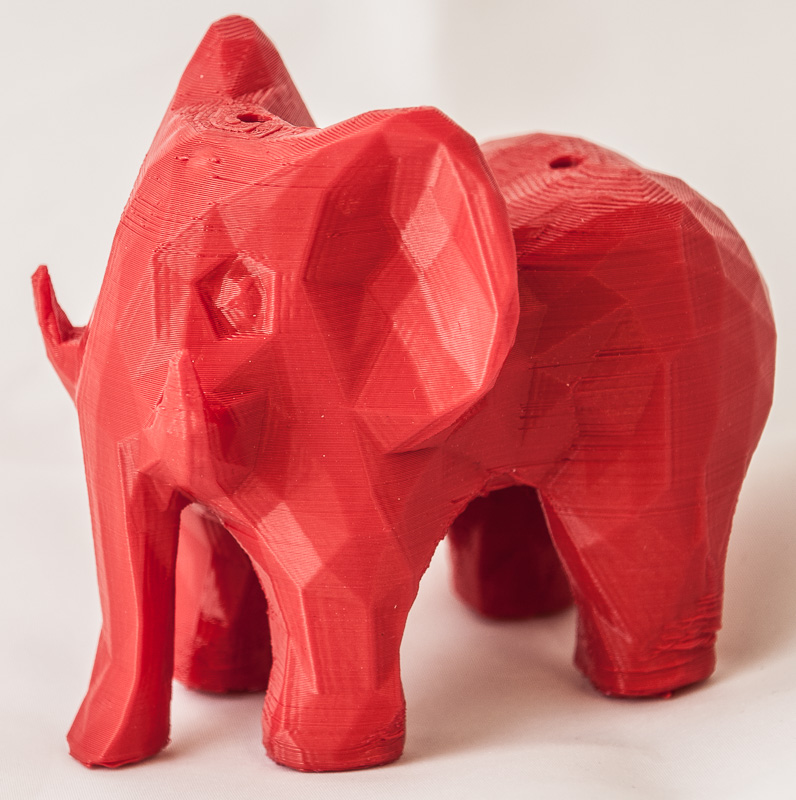
\includegraphics[height=.197\textwidth]{figures/elephant}}
      \subfloat[]{\label{fig:bar_rand}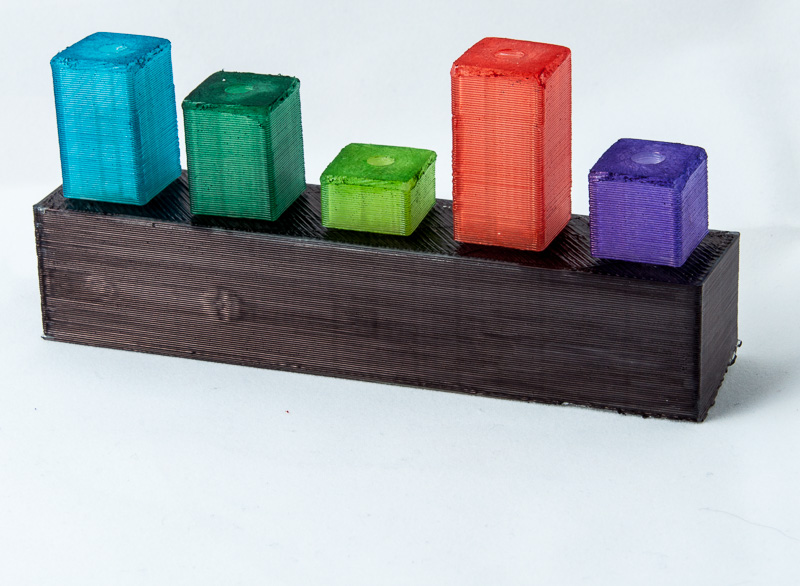
\includegraphics[height=.197\textwidth]{figures/bar_rand1}}
      \subfloat[]{\label{fig:whales}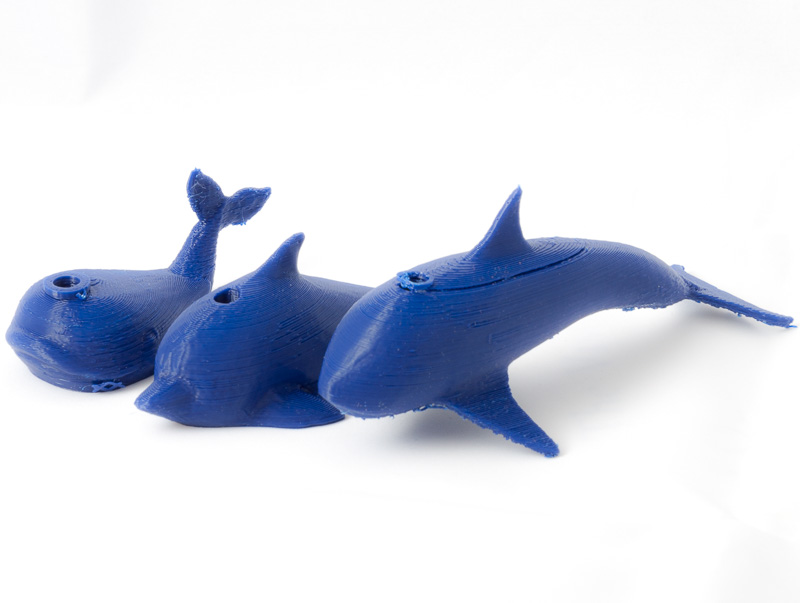
\includegraphics[height=.197\textwidth]{figures/whales}}
      \subfloat[]{\label{fig:cell}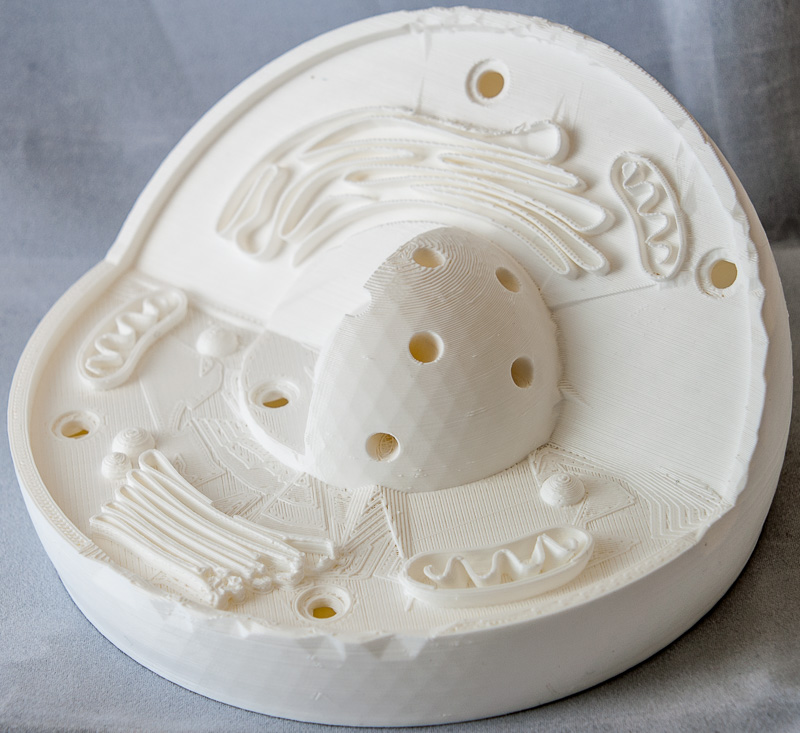
\includegraphics[height=.197\textwidth]{figures/cell}}
      \caption{Example \bh applications. The elephant \protect\subref{fig:elephant}
      has six holes (one on the head, one on the back, one on each foot) which,
      when blown into, activate text-to-speech with different elephant facts. Each
      bar in the bar chart \protect\subref{fig:bar_rand} triggers a readout of the
      quantity, and can be moved to represent different data. The sperm whale,
      dolphin, and orca \protect\subref{fig:whales} each produce a different tone
      to trigger videos of those animals. The cell model's blowholes interact with
      a quiz program to test knowledge of its components
      \protect\subref{fig:cell}.}%
      \label{fig:blowhole_demo}%
  }


  \maketitle

  \begin{abstract}
    Lorem ipsum dolor sit amet, consectetur adipiscing elit. Proin tempor placerat dictum. Maecenas sed mi sit amet dui lacinia lacinia sit amet nec enim. Nulla vitae arcu libero. Nunc sed arcu faucibus, aliquet mi ut, dictum elit. Aliquam semper in tellus tristique gravida. Vivamus sed orci at diam efficitur vulputate quis nec nisi. Suspendisse a lacus at velit semper cursus in id risus. Nunc elementum non orci eget venenatis. Praesent accumsan nibh quis tellus pulvinar, eget molestie enim lobortis. Sed id auctor leo. Morbi efficitur id nibh vel egestas. Suspendisse id scelerisque dui. Nam lacinia id velit eu venenatis. Proin interdum, nisi laoreet efficitur volutpat, sem libero auctor nibh, quis tristique nunc risus eget nunc.
  \end{abstract}

  \category{H.5.3.}{}{}\category{}{}{}
  \keywords{\plainkeywords}

  \section{Introduction}

  \section{Related Work}
    \subsection{Augmented Fabrication (?)}
    \subsection{Interactivity}
      \subsubsection{Acoustic}
      \subsubsection{Electric}
      \subsubsection{Hydraulic}
      \subsubsection{Optic}
      \subsubsection{Pneumatic}
      \subsubsection{Metamaterial}
    \subsection{Programming by Demonstration (?)}
          
  \section{Research Plan}
  	\section{Interactivity Toolkit}
  	\subsubsection{Blowhole}
  	  \textbf{Overview}\\
  	  \textbf{Implementation}\\  	  
  	  \textbf{Future Work}
  	\subsubsection{AirTouch}
  	\subsubsection{Shape-changing interfaces}

          
  \section{Conclusion}
            
  \section{Appendix}

  \bibliographystyle{SIGCHI-Reference-Format}
  \bibliography{papers,blowhole}

\end{document}